\chapter{Messungen} \label{Messungen}

Das nachfolgende Kapitel legt die Ergebnisse der Messungen dar. 



\section{Charakteisierung des Wandlers}

Die Ermittlung des Impedanzganges ist in \autoref{img:Impedanzgang} dargestellt. Hierbei wurde ein Serienwiederstand von \SI{51}{\Omega} verwendet.


\begin{figure}[h]
    \centering
    \includesvg[width=1 \textwidth]{Berechnungen/Impedanzgang.svg}
    \caption{Impedanzgang des Piezowandlers}
    \label{img:Impedanzgang}
\end{figure}


Die genaue Untersuchung der Impedanz unterhalb der ersten Resonanz ist in \autoref{img:Impedanzgang_unten} dargestellt. Hierbei wird der Impedanzgang mit \SI{51}{\Omega} und \SI{2200}{\Omega} gegenübergestellt.

\begin{figure}[h]
    \centering
    \includesvg[width=1 \textwidth]{Berechnungen/Impedanzgang_unten.svg}
    \caption{Impedanzgang unterhalb der ersten Resonanz}
    \label{img:Impedanzgang_unten}
\end{figure}




\section{Messung der Schallgeschwindigkeit} \label{Aufbau_Schall}
Zur Messung der Schallgeschwindigkeit wird im ersten Versuchsaufbau ein Probenkörper mit der Breite \SI{30}{mm} verwendet. Die Dicke des Piezos beträgt  \SI{2}{mm}. Es ergibt sich eine Laufzeit von \SI{6.1e-6}{s}. Beim zweiten Versuch eribt die Laufzeit \SI{10.3e-6}{s}.
Über den Zusammenhang  \(c=\frac{\lambda}{T}\) ergeben sich die Ausbreitungsgeschwindigkeiten zu :

\begin{equation*}
    \begin{split}
    c = \frac{\lambda}{T} = \frac{32 mm}{6.1e-6 s} = 5245.90 \frac{m}{s}  \\[.4cm]
    c = \frac{62 mm}{6.1e-6 s} = 6019.41 \frac{m}{s}  
    \end{split}
\end{equation*}




\section{Materialprüfung}

Die nachfolgende Tabelle stellt die Laufzeit der einzelnen Probekörpern bei unterschiedlichen Frequnezen gegnüber. 


\begin{table}[H]
    \centering
    \begin{tabular}{l|llll}
         Probekörper Nr. &  \SI{800}{kHz} & \SI{1}{MHz} & \SI{1.4}{MHz} &  \\
         \hline
         1 & 5.58  & 6.1  & 5.38 &   \\
         2 & 5.30  & 5.50 & 5.42 &  \\
         3 & 5.52  & 5.46 & 5.38 &  
    \end{tabular}
    \caption{Laufzeitmessung bei unterschiedlichen Frequnezen und Empfangsamplitude}
    \label{tab:Materialprüfung}
\end{table}


\autoref{img:Materialprufung} stellt die Laufzeitmessungen der Körper gegenüber. Dabei weisen die Amplitudenantworten abhängig vom Körper deutliche unterschiede auf.


\begin{figure}[h]
    \begin{minipage}[b]{.50\linewidth} % [b] => Ausrichtung an \caption
       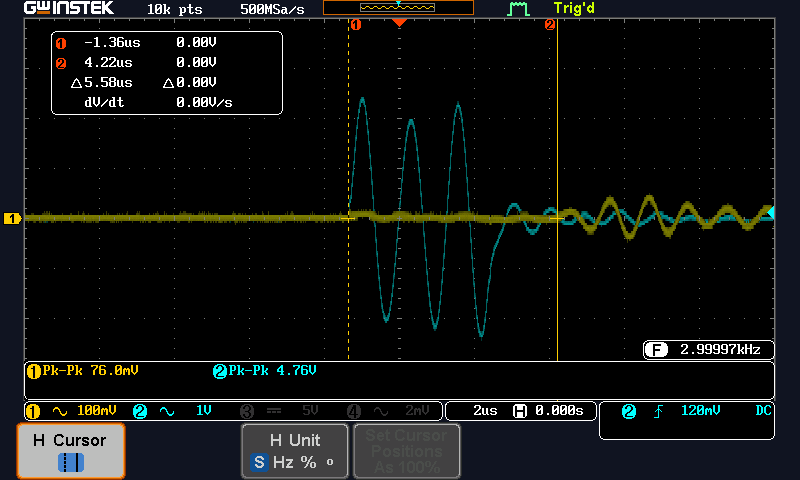
\includegraphics[width=\linewidth]{image/1_Quer.PNG}
       \caption*{\textbf{a)} Probekörper 1}
    \end{minipage}
    \hspace{.01\linewidth}% Abstand zwischen Bilder
    \begin{minipage}[b]{.5\linewidth} % [b] => Ausrichtung an \caption
       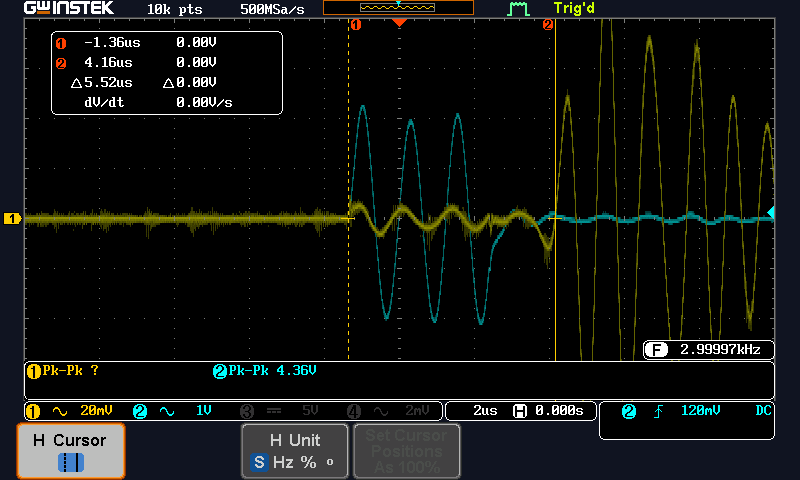
\includegraphics[width=\linewidth]{image/2_quer.PNG}
       \caption*{\textbf{b)} Probekörper 2}
    \end{minipage}

    \begin{minipage}[b]{.50\linewidth} % [b] => Ausrichtung an \caption
        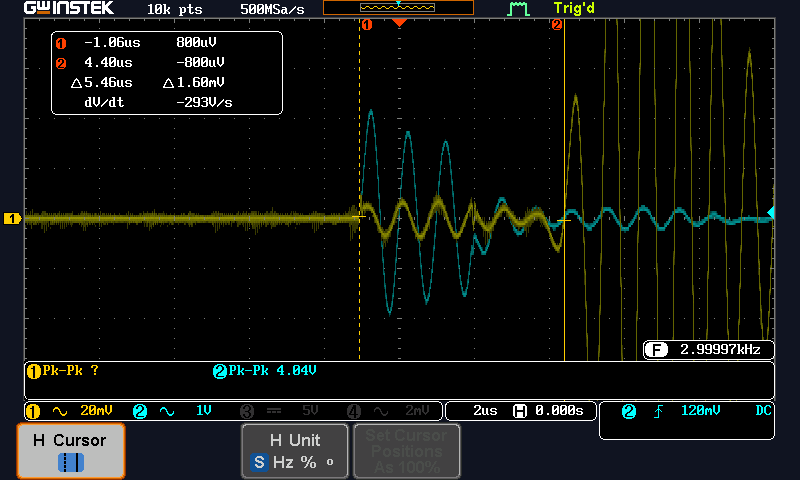
\includegraphics[width=\linewidth]{image/3_quer.PNG}
        \caption*{\textbf{a)} Probekörper 3}
     \end{minipage}
     \hspace{.01\linewidth}% Abstand zwischen Bilder
     
    \caption{Gegenüberstellung der Laufzeitmessung bei einer Anregung von \(V_{pp}= \SI{5}{V}, f= \SI{1}{MHz}\)}
    \label{img:Materialprufung}
 \end{figure}